\subsection{GERENTE DE CONSOLIDAÇÃO}

Para efetuar a consolidação, o agente proposto por \citeonline{gabriel} será adaptado para funcionar com a plataforma multiagente. Para tal, as tarefas efetuadas pelo agente proposto serão divididas entre quatro agentes:
\begin{itemize}
  \item Um gerente de consolidação encarregado de tomar decisões relativas a quais \emph{clusters} serão consolidados, mandar consolidá-los e marcá-los como consolidados;
	\item Um agente de consolidação encarregado de mapear VMs a servidores específicos e efetuar a migração de VMs para outros servidores para viabilizar a consolidação;
	\item Um gerente de alocação encarregado de tomar decisões realativas a alocação de novas VMs como onde alocá-las e a necessidade ou não de ativar recursos desligados;
	\item Um agente de alocação encarregado de concretizar as decisões do gerente de alocação, alocando VMs e ligando recursos desativados.
\end{itemize}

O gerente de consolidação, como mostrado na figura, irá escolher um \emph{cluster} para avaliar e determinar a possibilidade de sua consolidação baseado em um algoritmo de consolidação que deve ser especificado pelo usuário do sistema. Ao determinar qual \emph{cluster} será avaliado, uma mensagem é encaminhada ao agente de alocação solicitando a consolidação deste \emph{cluster} para que o agente posso avaliar e se possível efetuar a consolidação.

A figura contém uma legenda válida para todos os diagramas de agentes que serão apresentados a seguir, explicitando o significado dos elementos dos diagramas.

\begin{figure}[!htb]
	\centering
	\caption{Legenda relativa aos diagramas dos modelos de agentes.}\label{fig:legenda-agentes}
	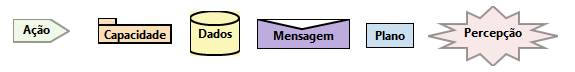
\includegraphics[width=1\textwidth]{figuras/legenda-agentes.png}
\end{figure}

\begin{figure}[!htb]
	\centering
	\caption{Modelo do Gerente de Consolidação.}\label{fig:gerente-consolidacao}
	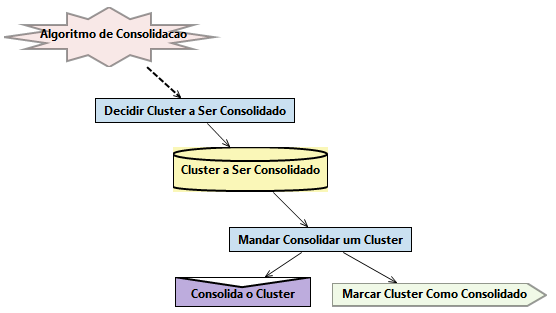
\includegraphics[width=1\textwidth]{figuras/gerente-consolidacao.png}
\end{figure}

\subsection{AGENTE DE CONSOLIDAÇÃO}

O agente de consolidação é o responsável por realizar todas as operações relacionadas a consolidação de um \emph{cluster}. Como explicitado na figura, ao receber a mensagem do gerente de consolidação solicitando a consolidação de um \emph{cluster}, o agente verifica os outros \emph{clusters} com servidores ativos e mapeia as VMs contidas no \emph{cluster} a ser consolidado para estes outros \emph{clusters} ativos, de acordo com a capacidade de cada um, visando mapear o maior número possível de VMs em um mesmo cluster de forma a não prejudicar o funcionamento das VMs submetendo-as a \emph{clusters} com recursos insuficientes disponíveis, comparando os recursos sendo utilizados no \emph{cluster} a ser consolidado aos recursos disponíveis no resto do ambiente. Assim que o maior número possível de VMs foi mapeado e migrado para servidores de outros \emph{clusters}, os servidores que então não possuem nenhuma VM mapeada a eles são desativados.

\begin{figure}[!htb]
	\centering
	\caption{Modelo do Agente de Consolidação.}\label{fig:agente-consolidacao}
	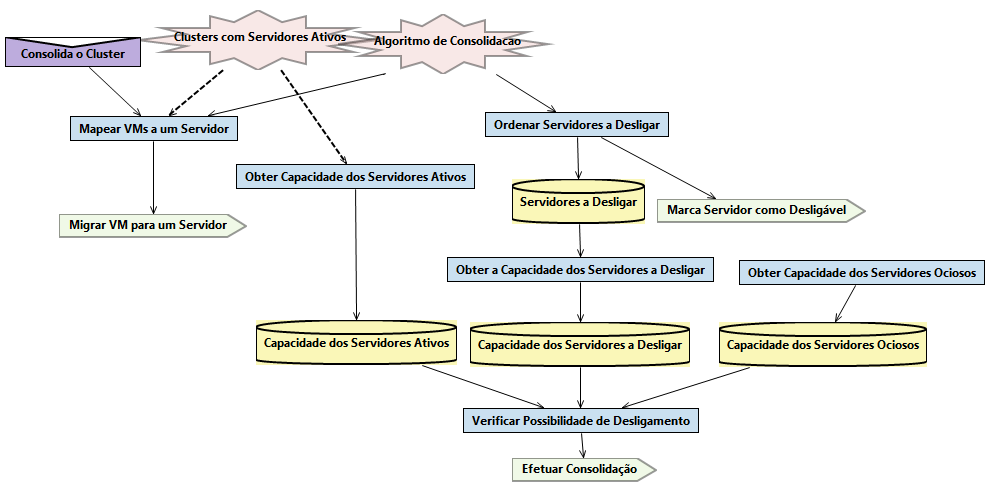
\includegraphics[width=1\textwidth]{figuras/agente-consolidacao.png}
\end{figure}

\subsection{GERENTE DE ALOCAÇÃO}

O gerente de alocação é o responsável por determinar onde novas VMs deverão ser alocadas. Quando uma nova VM é instanciada por um usuário, os \emph{clusters} disponíveis são ranquedos em uma ordem de acordo com um algoritmo de alocação que deve ser especificado pelo usuário da plataforma. Uma vez ordenados os \emph{clusters} o gerente de alocação envia uma mensagem ao agente de alocação para que tente realizar a alocação da nova VM. Porém, pode ser que não seja possível realizar a alocação em um dos \emph{clusters} especificados, possivelmente por falta de recursos disponíveis, ou mesmo pelo motivo de recursos ociosos terem sido consolidados previamente. Nesse caso, o agente de alocação retornará uma mensagem para o gerente informando a impossibilidade de alocar a VM, e o gerente tentará encontrar recursos extras que tenham sido consolidados. Existindo estes recursos, eles são ordenados de acordo com os interesses do usuário, e uma solicitação é encaminhada ao agente de alocação para que ele tente reativar recursos suficientes para alocar a VM. As figuras mostram o modelo das funcionalidades do gerente de alocação.

\begin{figure}[!htb]
	\centering
	\caption{Modelo do Gerente de Alocação.}\label{fig:gerente-alocacao1}
	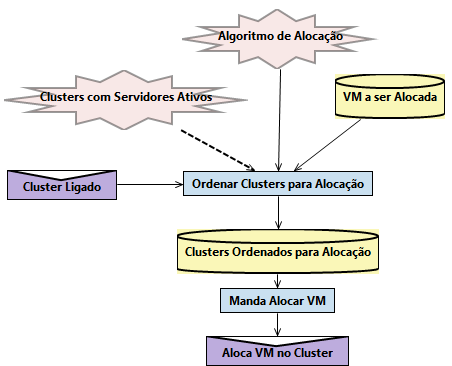
\includegraphics[width=1\textwidth]{figuras/gerente-alocacao1.png}
\end{figure}

\begin{figure}[!htb]
	\centering
	\caption{Modelo do Gerente de Alocação.}\label{fig:gerente-alocacao2}
	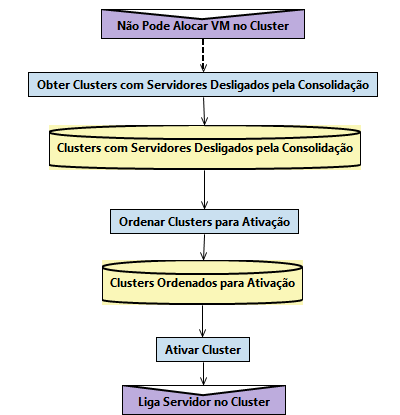
\includegraphics[width=1\textwidth]{figuras/gerente-alocacao2.png}
\end{figure}

\subsection{AGENTE DE ALOCAÇÃO}

O agente de alocação é o responsável por realizar as operações relacionadas à alocação de novas VMs. Ao receber a mensagem do gerente de alocação solicitando a alocação de uma VM, a agente procura recursos disponíveis para alocá-la nos \emph{clusters} na ordem especificada e ao encontrar um servidor capaz de suportá-la, realiza o mapeamento da VM a esse servidor. O agente pode também constatar a falta de recursos suficientes para alocar a VM solicitada. Quando isso acontecer, ele deve notificar o gerente de alocação para que sejam especificados os servidores desativados que o agente deve tentar reativar. Uma vez recebida a resposta do gerente, o agente tenta realizar a ativação dos recursos solicitados e, obtendo sucesso, avisa o gerente para que a alocação possa prosseguir normalmente. O modelo do agente de alocação é explicitado na figura.

\begin{figure}[!htb]
	\centering
	\caption{Modelo do Agente de Alocação.}\label{fig:agente-alocacao}
	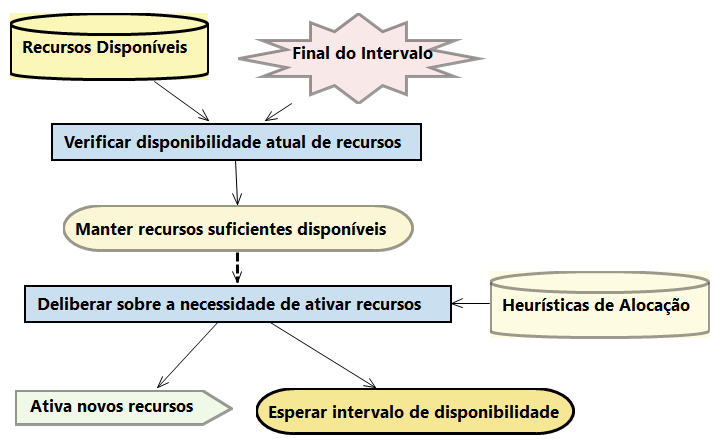
\includegraphics[width=1\textwidth]{figuras/agente-alocacao.png}
\end{figure}